\chapter{Statistical Analysis}
\label{chap:Results}

%%%%%%%%%%%%%%%%%%%%%%%%%%%%%%%%%%%%%%%%%%%%%%%%%%%%%%%%%%%%%
%%%%%%%%%%%%%%%%%%%%%%%%%%%%%%%%%%%%%%%%%%%%%%%%%%%%%%%%%%%%%
\section{Profile Likelihood Fit}
\label{sec:PLF}

A binned likelihood function $\mathcal{L}(\mu, \theta)$ is constructed to perform the statistical analysis on the BDT discriminator distributions. The parameter of interest (POI), denoted by $\mu$, is the signal strength that governs the cross section of the ST and TT signals simultaneously. All the uncertainties are incorporated into the likelihood function as nuisance parameters, denoted by $\theta$. The uncertainties that affect the shape of the BDT discriminator distributions are considered with Gaussian distributions while other uncertainties that only affect the normalizations are considered with log-normal distributions. 

To control the systematic uncertainties, a profile likelihood fit is performed simultaneously in six regions (three data-taking years and two signal regions) by maximizing the likelihood function $\mathcal{L}(\hat{\mu}, \hat{\theta})$. Both $\hat{\mu}$ and $\hat{\theta}$ are the maximum likelihood estimators for the signal strength and nuisance parameters, respectively. The scaling of the signal for the purpose of a better visualization is optimized based on ``VecU" signal, and it is kept the same for the other signals to compare their cross sections relative to each other. The post-fit distributions of the BDT discriminator are shown in Fig.~\ref{fig:bdt_postfit_VecU}-\ref{fig:bdt_postfit_ScalarC}. The most prominent uncertainties affecting the likelihood fit are the statistical uncertainties on MC samples.

\begin{figure}[tbh!]
 \begin{center}
 \begin{tabular}{cc}
  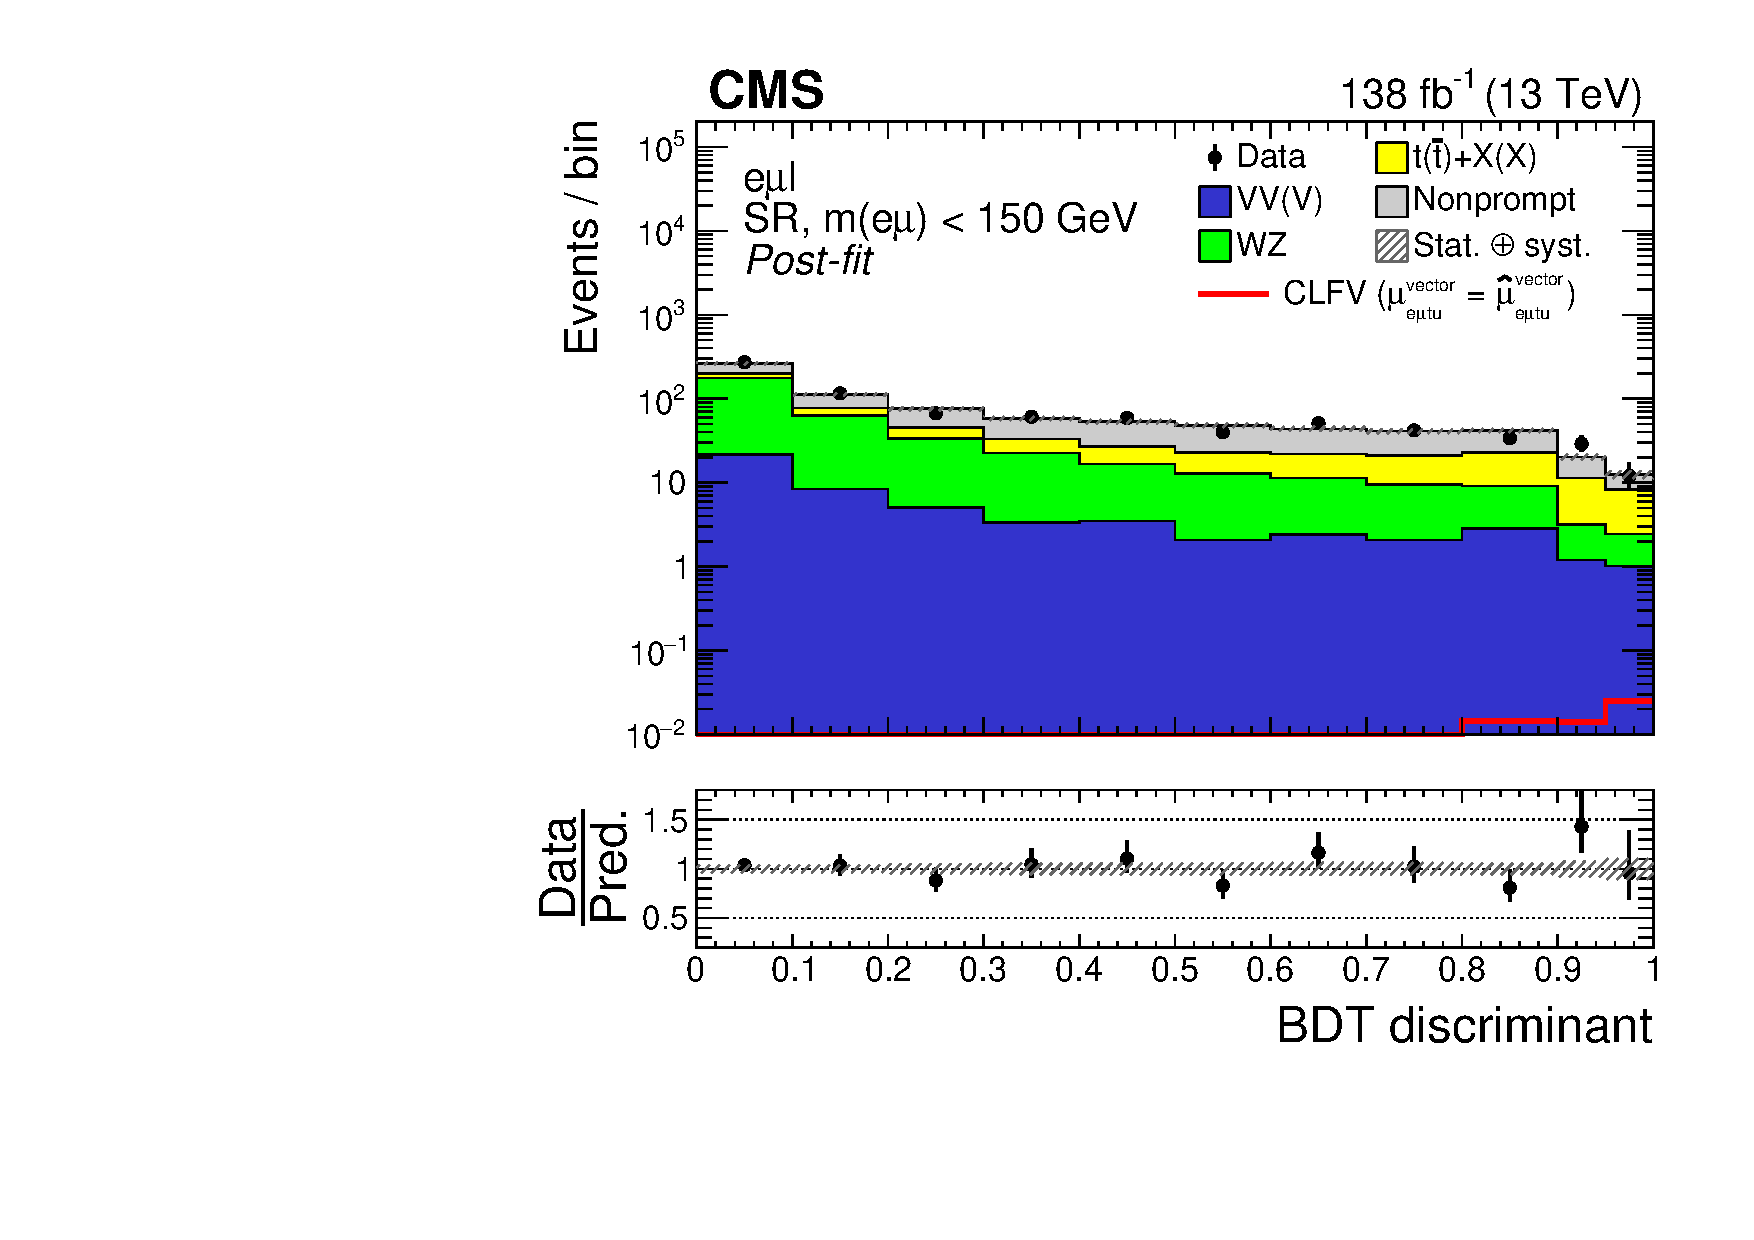
\includegraphics[width=0.48\textwidth]{figures/Part3/Results/BDT_TT_VecU}&
  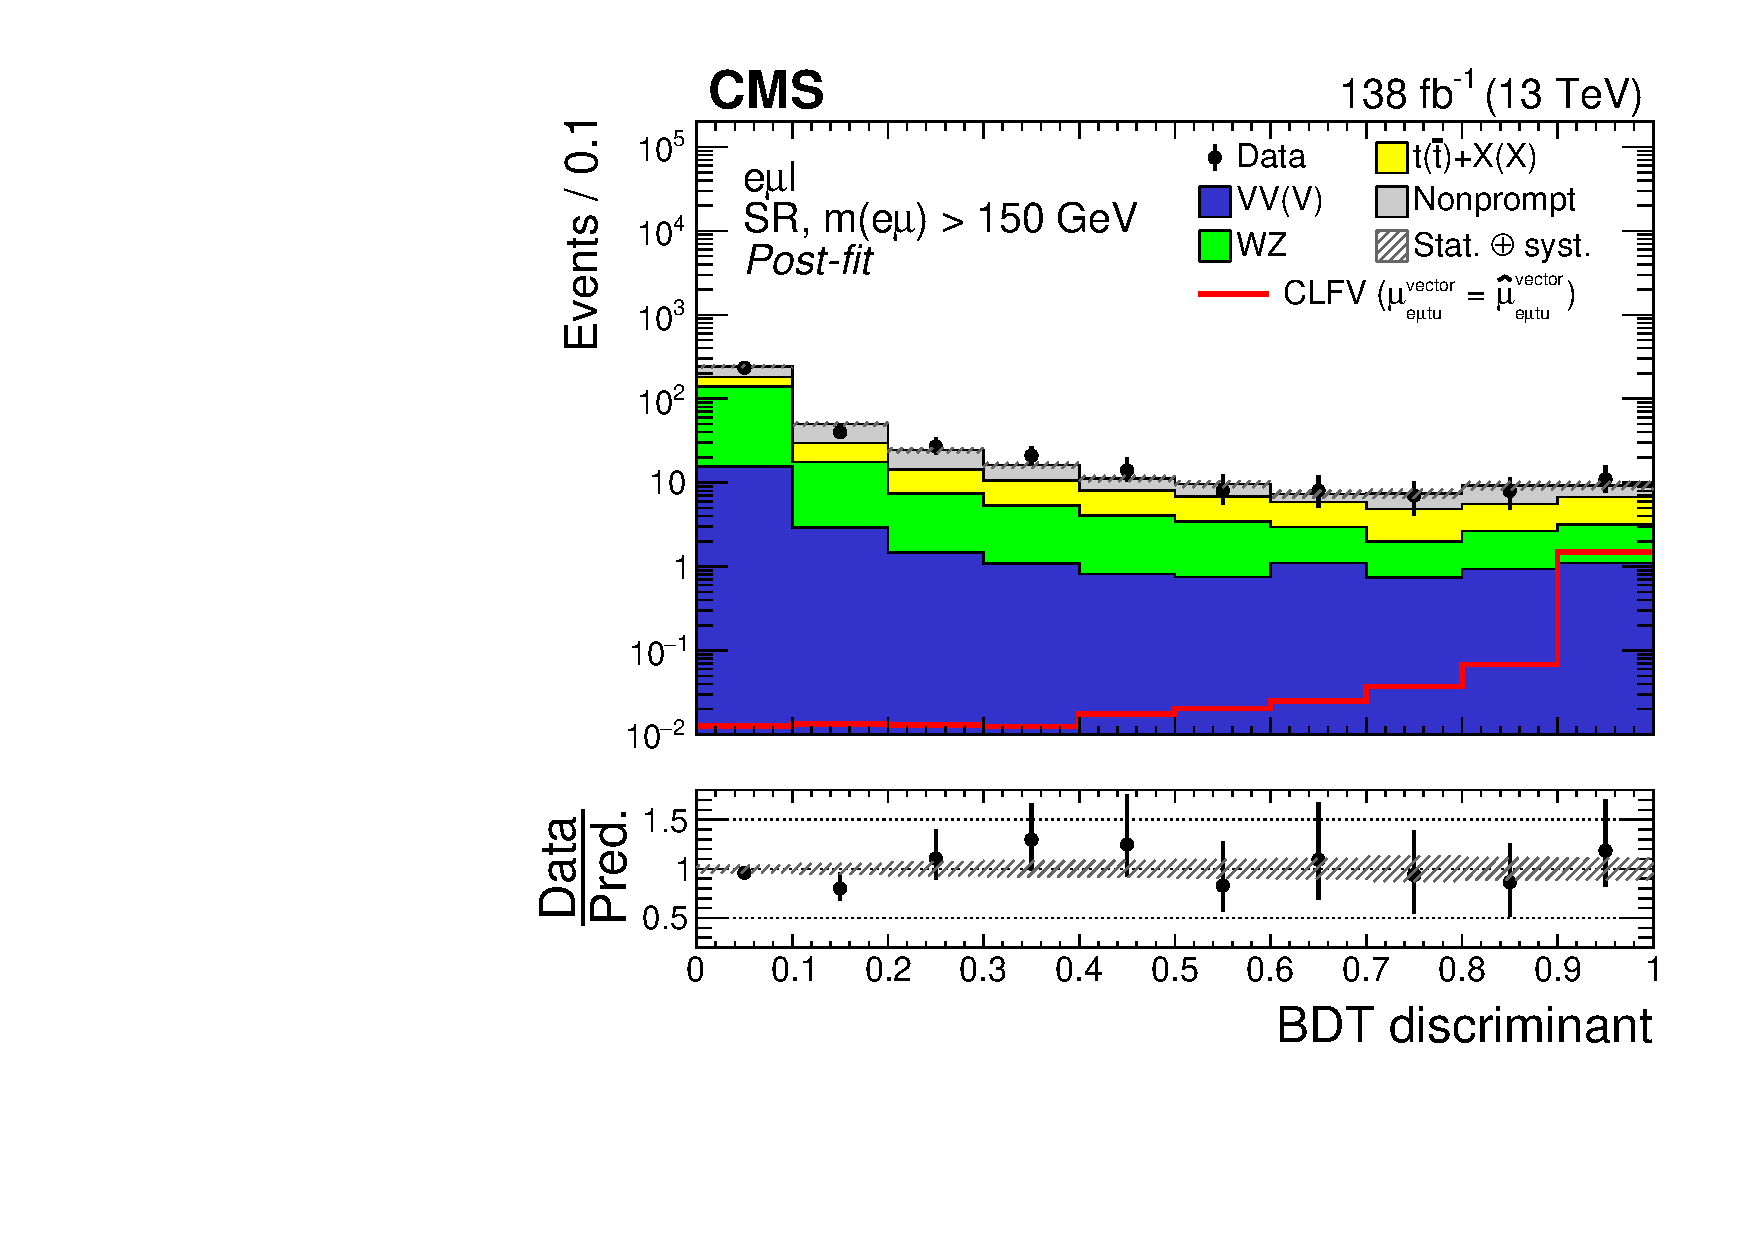
\includegraphics[width=0.48\textwidth]{figures/Part3/Results/BDT_ST_VecU}\\
 \end{tabular}
 \caption{Distributions of the posterior BDT discriminator distributions for the TT-enriched SR (left) and the ST-enriched SR (right). Signals are generated with vector-like operator involving an Up quark. The three data-taking years are aggregated for better visualization.}
 \label{fig:bdt_postfit_VecU}
 \end{center}
\end{figure} 
%%%%%%%%%%%%%%%%%%%%%%%%%%%%%%%%%%%%%%%%%%%%%%%%%%%%%%%%%%%%%
%%%%%%%%%%%%%%%%%%%%%%%%%%%%%%%%%%%%%%%%%%%%%%%%%%%%%%%%%%%%%
\section{Upper Limits}
\label{sec:Limits}

The results for the one-dimensional limits are summarized in Table~\ref{tab:limit}. Assuming a linear relationship between $\mathcal{B}(\tto{c})$ and $\mathcal{B}(\tto{c})$ in the case of nonvanishing signals, the two-dimensional limits can also be obtained through interpolation (see Fig.~\ref{fig:2dlimit}). This analysis constitutes the most stringent limits on these processes to date.

\begin{table}[th]
\sffamily
\centering
\resizebox{0.95\linewidth}{!}{%
\begin{tabular}{cccccc}
\toprule
CLFV  & Lorentz  & \multicolumn{2}{c}{$\WC{}{\emut{q}}/\mathrm{\Lam}^2~(\TeV^{-2})$} & \multicolumn{2}{c}{$\mathcal{B} (\tto{q}) \times 10^{-6}$} \\
coupling  & structure & exp (68\% range) & obs & exp (68\% range) & obs \\
\midrule
\multirow{3}{*}{$\emut{u}$}& tensor  & 0.022 (0.018--0.026) & \textbf{0.024} & 0.027 (0.018--0.040) & \textbf{0.032}\\
& vector & 0.044 (0.036--0.054) & \textbf{0.048} & 0.019 (0.013--0.028) & \textbf{0.022}\\
& scalar & 0.093 (0.077--0.114) & \textbf{0.101} & 0.010 (0.007--0.016) & \textbf{0.012}\\
\midrule
\multirow{3}{*}{$\emut{c}$} & tensor & 0.084 (0.069--0.102) & \textbf{0.094} & 0.396 (0.272--0.585) & \textbf{0.498}\\
 & vector & 0.175 (0.145--0.214) & \textbf{0.196} & 0.296 (0.203--0.440) & \textbf{0.369}\\
 & scalar & 0.385 (0.318--0.471) & \textbf{0.424} & 0.178 (0.122--0.266) & \textbf{0.216}\\
 \bottomrule
\end{tabular}
}
\caption{Upper limit on the LFV signal using the full Run 2 data set.}
\label{tab:limit}
\end{table}

\begin{figure}[tbh!]
 \begin{center}
 \begin{tabular}{cc}
  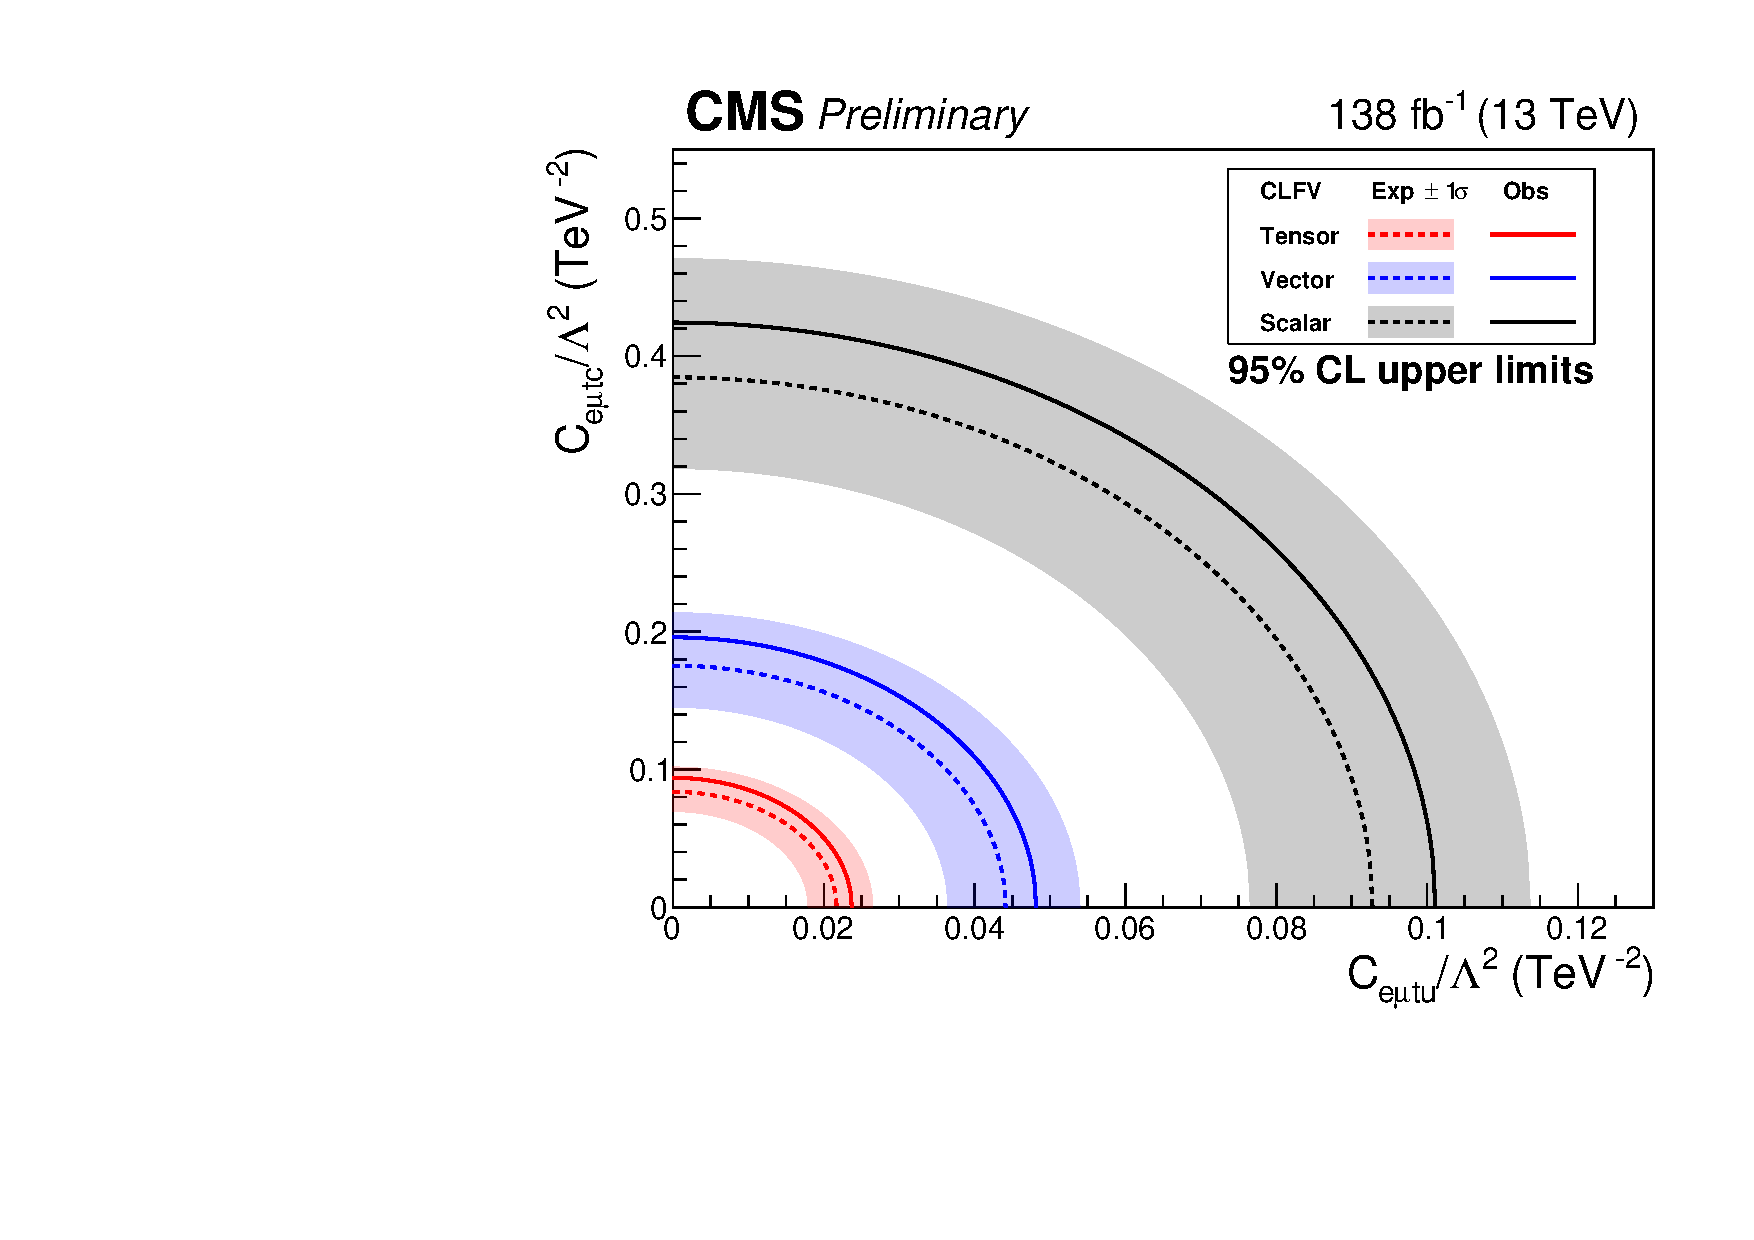
\includegraphics[width=0.48\textwidth]{figures/Part3/Results/Hist2D_WC}&
  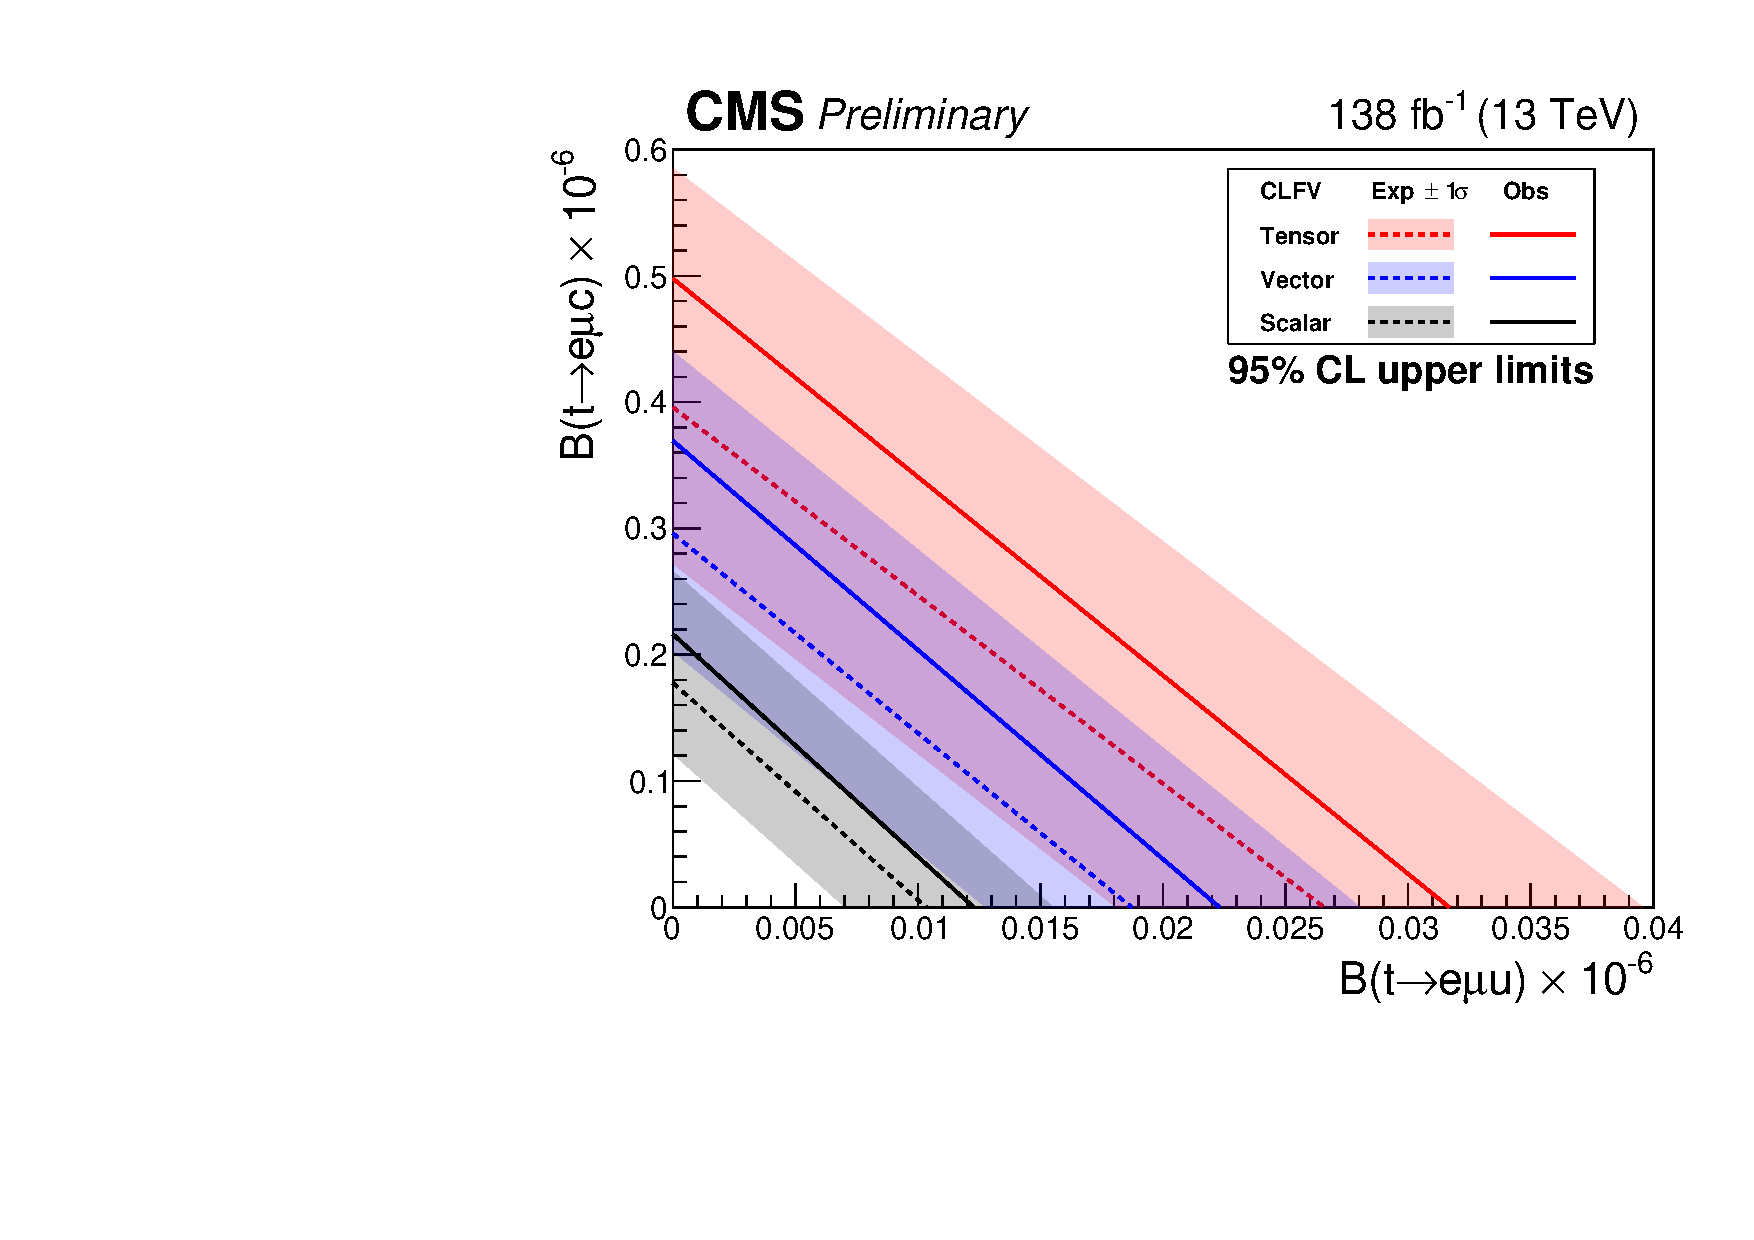
\includegraphics[width=0.48\textwidth]{figures/Part3/Results/Hist2D_BR}\\
 \end{tabular}
 \caption{Two-dimensional upper limits on the Wilson coefficients (left) and the branching ratios (right).}
 \label{fig:2dlimit}
 \end{center}
\end{figure}